% Convert with command:
% convert -density 300 pic.pdf -quality 90 pic.png
\documentclass[crop,tikz,border=0pt]{standalone}
\usetikzlibrary{arrows.meta, fit}
\begin{document}

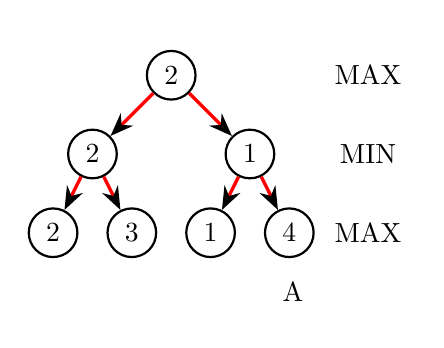
\begin{tikzpicture}
\begin{scope}[every node/.style={circle,thick,draw}]
    \node (1) at (0, 0) [shape=circle,draw=black,fill=white] {2};

    \node (2) at (-1, -1) [shape=circle,draw=black,fill=white] {2};
    \node (3) at (1, -1) [shape=circle,draw=black,fill=white] {1};

    \node (4) at (-1.5, -2) [shape=circle,draw=black,fill=white] {2};
    \node (5) at (-0.5, -2) [shape=circle,draw=black,fill=white] {3};

    \node (6) at (0.5, -2) [shape=circle,draw=black,fill=white] {1};
    \node (7) at (1.5, -2) [shape=circle,draw=black,fill=white] {4};
    \draw[] (1.8, -2.5) node[draw=white,below left] {A};

    \node (max1) at (2.5, 0) [shape=circle,draw=white,fill=white] {MAX};
    \node (min) at (2.5, -1) [shape=circle,draw=white,fill=white] {MIN};
    \node (max2) at (2.5, -2) [shape=circle,draw=white,fill=white] {MAX};
\end{scope}

\begin{scope}[>={Stealth[black]},
            %   every node/.style={fill=white,rectangle,above},
              every edge/.style={draw=red,very thick}]
    \path [->] (1) edge node {} (2);
    \path [->] (1) edge node {} (3);

    \path [->] (2) edge node {} (4);
    \path [->] (2) edge node {} (5);

    \path [->] (3) edge node {} (6);
    \path [->] (3) edge node {} (7);
\end{scope}
\end{tikzpicture}

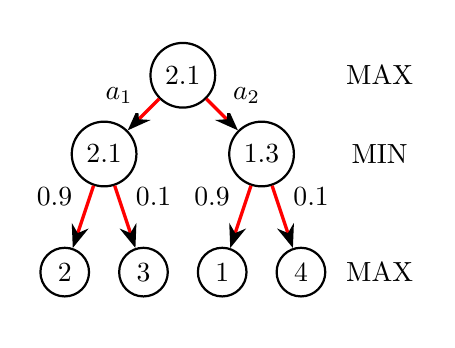
\begin{tikzpicture}
\begin{scope}[every node/.style={circle,thick,draw}]
    \node (1) at (0, 0) [shape=circle,draw=black,fill=white] {2.1};

    \node (2) at (-1, -1) [shape=circle,draw=black,fill=white] {2.1};
    \node (3) at (1, -1) [shape=circle,draw=black,fill=white] {1.3};

    \node (4) at (-1.5, -2.5) [shape=circle,draw=black,fill=white] {2};
    \node (5) at (-0.5, -2.5) [shape=circle,draw=black,fill=white] {3};

    \node (6) at (0.5, -2.5) [shape=circle,draw=black,fill=white] {1};
    \node (7) at (1.5, -2.5) [shape=circle,draw=black,fill=white] {4};

    \node (max1) at (2.5, 0) [shape=circle,draw=white,fill=white] {MAX};
    \node (min) at (2.5, -1) [shape=circle,draw=white,fill=white] {MIN};
    \node (max2) at (2.5, -2.5) [shape=circle,draw=white,fill=white] {MAX};
\end{scope}

\begin{scope}[>={Stealth[black]},
            %   every node/.style={fill=white,rectangle,above},
              every edge/.style={draw=red,very thick}]
    \path [->] (1) edge node[fill=white,above left] {$a_1$} (2);
    \path [->] (1) edge node[fill=white,above right] {$a_2$} (3);

    \path [->] (2) edge node[fill=white,above left] {0.9} (4);
    \path [->] (2) edge node[fill=white,above right] {0.1} (5);

    \path [->] (3) edge node[fill=white,above left] {0.9} (6);
    \path [->] (3) edge node[fill=white,above right] {0.1} (7);
\end{scope}
\end{tikzpicture}

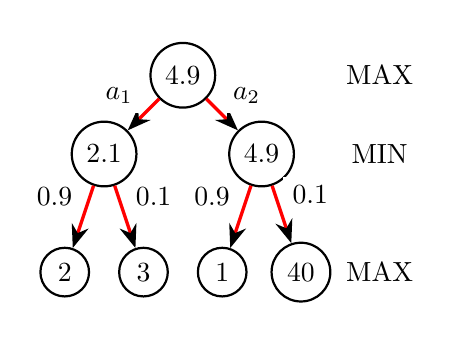
\begin{tikzpicture}
\begin{scope}[every node/.style={circle,thick,draw}]
    \node (1) at (0, 0) [shape=circle,draw=black,fill=white] {4.9};

    \node (2) at (-1, -1) [shape=circle,draw=black,fill=white] {2.1};
    \node (3) at (1, -1) [shape=circle,draw=black,fill=white] {4.9};

    \node (4) at (-1.5, -2.5) [shape=circle,draw=black,fill=white] {2};
    \node (5) at (-0.5, -2.5) [shape=circle,draw=black,fill=white] {3};

    \node (6) at (0.5, -2.5) [shape=circle,draw=black,fill=white] {1};
    \node (7) at (1.5, -2.5) [shape=circle,draw=black,fill=white] {40};

    \node (max1) at (2.5, 0) [shape=circle,draw=white,fill=white] {MAX};
    \node (min) at (2.5, -1) [shape=circle,draw=white,fill=white] {MIN};
    \node (max2) at (2.5, -2.5) [shape=circle,draw=white,fill=white] {MAX};
\end{scope}

\begin{scope}[>={Stealth[black]},
            %   every node/.style={fill=white,rectangle,above},
              every edge/.style={draw=red,very thick}]
    \path [->] (1) edge node[fill=white,above left] {$a_1$} (2);
    \path [->] (1) edge node[fill=white,above right] {$a_2$} (3);

    \path [->] (2) edge node[fill=white,above left] {0.9} (4);
    \path [->] (2) edge node[fill=white,above right] {0.1} (5);

    \path [->] (3) edge node[fill=white,above left] {0.9} (6);
    \path [->] (3) edge node[fill=white,above right] {0.1} (7);
\end{scope}
\end{tikzpicture}

\end{document}
